% TradeBot: a reader's guide to the project.
% Build (MiKTeX): pdflatex -aux-directory=<tmp> tradebot-guide.tex   (run twice for the contents page)
\documentclass[11pt,a4paper]{article}

% ---------- fonts & encoding ----------
\usepackage[T1]{fontenc}
\usepackage[utf8]{inputenc}
\usepackage{XCharter}
\usepackage[xcharter]{newtxmath}
\usepackage[scaled=0.88]{FiraSans}
\usepackage[scaled=0.9,varqu]{inconsolata}
\usepackage{textcomp}
\DeclareUnicodeCharacter{2192}{\ensuremath{\rightarrow}}
\DeclareUnicodeCharacter{2264}{\ensuremath{\le}}
\DeclareUnicodeCharacter{2265}{\ensuremath{\ge}}
\DeclareUnicodeCharacter{2248}{\ensuremath{\approx}}
\DeclareUnicodeCharacter{2212}{\ensuremath{-}}
\DeclareUnicodeCharacter{03C3}{\ensuremath{\sigma}}

% ---------- layout ----------
\usepackage[a4paper,left=2.4cm,right=2.4cm,top=2.5cm,bottom=2.6cm,headsep=0.9cm]{geometry}
\usepackage{microtype}
\usepackage{parskip}
\usepackage{graphicx}
\usepackage{xcolor}
\usepackage{tikz}
\usetikzlibrary{arrows.meta,positioning,calc,fit,backgrounds,shapes.geometric,shapes.symbols}
\usepackage[skins,breakable,raster]{tcolorbox}
\usepackage{tabularx,array,longtable}
\usepackage{enumitem}
\usepackage{titlesec}
\usepackage{fancyhdr}
\usepackage{amsmath}
\usepackage{pifont}
\usepackage{needspace}
\usepackage{multicol}
\usepackage[colorlinks=true,linkcolor=accent,urlcolor=teal,citecolor=accent,bookmarksnumbered=true]{hyperref}

% ---------- colours ----------
\definecolor{ink}{HTML}{1F2937}
\definecolor{accent}{HTML}{1D4E89}
\definecolor{teal}{HTML}{0F766E}
\definecolor{good}{HTML}{15803D}
\definecolor{bad}{HTML}{B91C1C}
\definecolor{warn}{HTML}{B45309}
\definecolor{muted}{HTML}{6B7280}
\definecolor{paper}{HTML}{F3F4F6}
\definecolor{purple}{HTML}{6D28D9}
\AtBeginDocument{\color{ink}}
\newcommand\euro{\ifmmode\text{\texteuro}\else\texteuro\fi}

% ---------- headings, header, lists ----------
\titleformat{\section}{\sffamily\LARGE\bfseries\color{accent}}{\thesection}{0.6em}{}
\titlespacing*{\section}{0pt}{3.2ex plus 1ex}{1.4ex}
\titleformat{\subsection}{\sffamily\large\bfseries\color{ink}}{\thesubsection}{0.6em}{}
\titlespacing*{\subsection}{0pt}{2.4ex plus .6ex}{0.8ex}
\titleformat{\subsubsection}{\sffamily\normalsize\bfseries\color{accent}}{}{0em}{}
\titlespacing*{\subsubsection}{0pt}{1.8ex plus .5ex}{0.4ex}
\newcommand\Section[1]{\Needspace{14\baselineskip}\section{#1}}

\setlength{\headheight}{14pt}
\pagestyle{fancy}
\fancyhf{}
\renewcommand\headrulewidth{0pt}
\renewcommand\sectionmark[1]{\markboth{\thesection\enspace #1}{}}
\fancyhead[L]{\sffamily\footnotesize\color{muted}TradeBot \textperiodcentered{} Reader's guide}
\fancyhead[R]{\sffamily\footnotesize\color{muted}\leftmark}
\fancyfoot[C]{\sffamily\footnotesize\color{muted}\thepage}

\setlist{itemsep=2pt,topsep=3pt,parsep=0pt}
\setlist[itemize]{label=\textcolor{accent}{\raisebox{0.15ex}{\scriptsize$\blacktriangleright$}},leftmargin=1.4em}
\setlist[enumerate]{label=\textcolor{accent}{\sffamily\bfseries\arabic*.},leftmargin=1.6em}

% ---------- tables ----------
\newcolumntype{L}{>{\raggedright\arraybackslash}X}
\newcolumntype{P}[1]{>{\raggedright\arraybackslash}p{#1}}
\newcommand\TopRule{\noalign{\hrule height 0.9pt\vskip 2pt}}
\newcommand\MidRule{\noalign{\vskip 1pt\hrule height 0.4pt\vskip 2pt}}
\newcommand\BotRule{\noalign{\vskip 2pt\hrule height 0.9pt}}
\newcommand\hd[1]{\textsf{\bfseries\small #1}}
\newenvironment{tbl}[1]
  {\par\smallskip\small\renewcommand\arraystretch{1.22}\tabularx{\linewidth}{#1}}
  {\endtabularx\par\medskip}

% ---------- small helpers ----------
\newcommand\code[1]{\texttt{#1}}
\newcommand\yes{\textcolor{good}{\ding{51}}}
\newcommand\no{\textcolor{bad}{\ding{55}}}
\newcommand\stag[2]{\textsf{\bfseries\footnotesize\textcolor{#1}{#2}}}
\newcommand\PASS{\stag{good}{PASS}}
\newcommand\FAIL{\stag{bad}{FAIL}}
\newcommand\WAIT{\stag{warn}{PENDING}}
\newcommand\LATER{\stag{muted}{LATER}}
\newcommand\doc[1]{\textsf{\footnotesize\textcolor{teal}{#1}}}

\newtcolorbox{callout}[2][accent]{enhanced,breakable,colback=#1!6,colframe=#1!6,boxrule=0pt,arc=0pt,
  borderline west={2.6pt}{0pt}{#1},left=10pt,right=10pt,top=7pt,bottom=7pt,before skip=8pt,after skip=10pt,
  before upper={{\sffamily\bfseries\color{#1}#2}\par\smallskip}}
\newtcolorbox{plainbox}[1][accent]{enhanced,breakable,colback=#1!6,colframe=#1!6,boxrule=0pt,arc=0pt,
  borderline west={2.6pt}{0pt}{#1},left=10pt,right=10pt,top=7pt,bottom=7pt,before skip=8pt,after skip=10pt}

\newcommand\tile[2]{%
  \begin{tcolorbox}[enhanced,colback=paper,colframe=paper,arc=2pt,boxrule=0pt,left=6pt,right=6pt,top=6pt,bottom=6pt,halign=left]
  {\sffamily\bfseries\Large\color{accent}#1}\par\vspace{2pt}{\sffamily\footnotesize\color{ink}#2}
  \end{tcolorbox}}

% ---------- TikZ styles ----------
\tikzset{
  box/.style={draw=#1,fill=#1!8,rounded corners=2pt,line width=0.7pt,align=center,
              font=\sffamily\scriptsize,inner sep=3pt,minimum height=1.05cm},
  box/.default=accent,
  arr/.style={-{Stealth[length=5pt,width=4pt]},line width=0.7pt,color=ink!80},
  darr/.style={-{Stealth[length=5pt,width=4pt]},line width=0.7pt,color=bad,dashed},
  lbl/.style={font=\sffamily\tiny,color=muted,align=center},
}

\begin{document}

% =====================================================================
% TITLE PAGE
% =====================================================================
\begin{titlepage}
\begin{tikzpicture}[remember picture,overlay]
  \fill[accent] (current page.north west) rectangle ([yshift=-11.5cm]current page.north east);
  \node[anchor=north west,text=white,font=\sffamily\bfseries\fontsize{44}{48}\selectfont]
    at ([xshift=2.4cm,yshift=-3.0cm]current page.north west) {TradeBot};
  \node[anchor=north west,text=white,font=\sffamily\LARGE]
    at ([xshift=2.4cm,yshift=-5.0cm]current page.north west) {A reader's guide to the project};
  \node[anchor=north west,text width=15.5cm,text=white!80!accent,font=\sffamily\large,align=left]
    at ([xshift=2.4cm,yshift=-6.3cm]current page.north west)
    {How a guarded, research-grade trading agent is designed, what it has shown so far, and what happens next.};
  % pipeline motif
  \begin{scope}[shift={([xshift=2.4cm,yshift=-9.6cm]current page.north west)},
                every node/.style={font=\sffamily\scriptsize,text=white,align=center}]
    \foreach \x/\t in {0/Data,2.55/Strategies,5.1/LLM desk,7.65/Risk engine,10.2/Execution,12.75/Broker}{
      \node[draw=white!70!accent,rounded corners=2pt,minimum width=2.1cm,minimum height=0.75cm] at (\x+1.05,0) {\t};
    }
    \foreach \a/\b in {0/2.55,2.55/5.1,5.1/7.65,7.65/10.2,10.2/12.75}{
      \draw[-{Stealth[length=4pt]},white!70!accent,line width=0.6pt] (\a+2.1,0) -- (\b,0);
    }
    \node[text=white!70!accent,font=\sffamily\tiny] at (6.15,-0.62) {reduce or veto only};
    \node[text=white!70!accent,font=\sffamily\tiny] at (8.7,-0.62) {every order checked};
  \end{scope}
\end{tikzpicture}

\vspace*{10.6cm}

{\sffamily
\begin{tabular}{@{}p{3.6cm}p{11cm}@{}}
\textcolor{muted}{Status as of} & \textbf{Monday, 28 September 2026}\\[3pt]
\textcolor{muted}{Phase} & \textbf{P1}: the demo engine runs 24/7 on the Trading 212 practice account\\[3pt]
\textcolor{muted}{Repository} & \code{github.com/kelvinvaddoriya/trade-bot-research}, commit \code{7b2f515}\\[3pt]
\textcolor{muted}{Based on} & \code{README.md}, \code{docs/01}--\code{10}, the source code, the configs and the reports in \code{reports/}\\
\end{tabular}}

\vfill

\begin{plainbox}[warn]
\small\textsf{\bfseries\color{warn}Not investment advice.} TradeBot is a research and engineering project. The project's own
documents stress that active retail traders tend to underperform passive investing after costs
(Barber \& Odean, 2000). The prototype is judged on engineering quality and honest measurement. It promises no returns,
and at a \euro1,000 cap a good year is worth tens of euros.
\end{plainbox}
\end{titlepage}

% =====================================================================
\pagenumbering{roman}
\setcounter{tocdepth}{2}
{\hypersetup{linkcolor=ink}\tableofcontents}
\clearpage
\pagenumbering{arabic}

% =====================================================================
\Section{The project on one page}
% =====================================================================

TradeBot is a \textbf{research prototype of an automated trading agent}. It trades a short whitelist of US and European
stocks and ETFs on a \textbf{Trading 212 practice (demo) account}, and it behaves as if it had at most \textbf{\euro1,000},
even though the demo account holds more. It is built to look and work like a proper production system, with a journal, a
risk engine, a kill switch and a watchdog, while being honest that at this size and with these strategies it is not a money
machine. What it is meant to prove is that the \emph{process} is sound: correct signals, controlled risk, and live behaviour
that matches the backtest.

\begin{callout}{The design in one sentence}
\emph{Deterministic strategies propose trades. A panel of five language models from five labs may only shrink or veto them, by
majority. An independent risk engine checks every order. A single execution service is the only thing that ever talks to
the broker.}
\end{callout}

\begin{tcbraster}[raster columns=4,raster equal height,raster column skip=6pt,raster row skip=6pt]
\tile{\euro1,000}{capital cap, identical in demo and in any later live phase}
\tile{20}{whitelisted instruments: 6 UCITS ETFs, 14 large-cap stocks}
\tile{S1 \yes\ \ S2 \no}{strategy S1 passed its backtest gate; S2 failed after costs}
\tile{5}{LLM jurors planned for the review desk (phase P2)}
\tile{82}{automated tests, all passing}
\tile{\textasciitilde2,400}{lines of Python in \code{src/tradebot/}}
\tile{5 of 8}{P1 safety drills passed live against the demo account}
\tile{P1}{current phase: demo engine running since 27 Sep, 23:02}
\end{tcbraster}

\subsection*{Where things stand}
\begin{itemize}
  \item \textbf{P0, foundations and backtest (done 25 Sep).} Data pipeline, indicators, two strategies, sizing, simulator,
        backtester and risk engine. \textbf{S1} (trend filter on ETFs) passed the gate; \textbf{S2} (pullback on stocks)
        failed because costs ate its small edge.
  \item \textbf{P1, the demo engine (built 27 Sep).} Order manager, reconciler, protective stops, kill switch, watchdog,
        alerts and daily report. Installed as Windows scheduled tasks on 27 Sep at 23:02 and running since.
        The demo run officially starts \textbf{today, 28 Sep}.
  \item \textbf{First real decision:} Wednesday 30 Sep after the Xetra close (S1's monthly check).
        \textbf{First orders:} Thursday 1 Oct at 09:02.
  \item \textbf{Next gate:} about two weeks of clean unattended running, plus the three drills that need a live position
        or the LLM desk.
\end{itemize}

\subsection*{How to read this guide}
\begin{tbl}{@{}P{2.2cm}L@{}}
\TopRule
\hd{Sections} & \hd{Answer the question} \\
\MidRule
2--3 & \emph{Why} is it built this way, and which decisions frame it? \\
4--6 & \emph{What} does it trade, where, and does it actually work? \\
7--8 & \emph{How} does the running system work, and how does it stay safe? \\
9    & What will the multi-model LLM desk do once it is built (P2)? \\
10--12 & Where does it run, how is the code organised, and how do you operate it? \\
13--14 & What happens next, and what do the terms mean? \\
\BotRule
\end{tbl}
Each section names the repository document with the full detail, like this: \doc{docs/04 §3}.

% =====================================================================
\Section{Why it is built this way}
% =====================================================================
\doc{docs/02-approaches.md}

\subsection{What ``agent'' means here}
The trading agent is the whole loop, not just an AI model:
\begin{center}
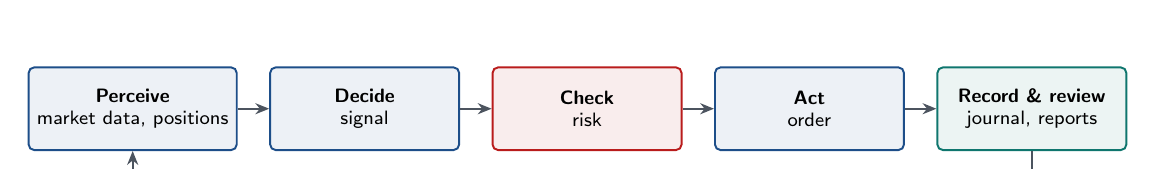
\begin{tikzpicture}[node distance=4mm]
  \node[box,minimum width=2.4cm] (a) {\textbf{Perceive}\\market data, positions};
  \node[box,minimum width=2.4cm,right=of a] (b) {\textbf{Decide}\\signal};
  \node[box=bad,minimum width=2.4cm,right=of b] (c) {\textbf{Check}\\risk};
  \node[box,minimum width=2.4cm,right=of c] (d) {\textbf{Act}\\order};
  \node[box=teal,minimum width=2.4cm,right=of d] (e) {\textbf{Record \& review}\\journal, reports};
  \foreach \p/\q in {a/b,b/c,c/d,d/e} \draw[arr] (\p) -- (\q);
  \draw[arr] (e.south) -- ++(0,-0.35) -| (a.south);
\end{tikzpicture}
\end{center}
An LLM could sit at several points of that loop. The central design question is therefore: \textbf{which component makes
the trade decision, and what is the LLM allowed to do?}

\subsection{Five ways to build a trading agent}
\begin{tbl}{@{}P{2.3cm}LLP{2.1cm}@{}}
\TopRule
\hd{Approach} & \hd{Strength} & \hd{Weakness that matters here} & \hd{Verdict} \\
\MidRule
A.\ Rule-based & Fully backtestable, deterministic, auditable, cheap; decades of research on trend and mean reversion &
  Small, widely known edges; parameters easy to overfit; blind to news & \textbf{the core} \\
B.\ ML prediction & Can combine many weak signals & Short, noisy, shifting data make overfitting the default & later research \\
C.\ Reinforcement learning & Optimises sizing and timing too & Sample-hungry; learns the simulator, not the market & no \\
D.\ LLM as trader & Reads news, explains itself & \textbf{Cannot be honestly backtested}; non-deterministic; prompt injection & no \\
E.\ Hybrid & Honest, testable core plus context from LLMs & The LLM's upside is limited, by design & \textbf{\color{good}chosen} \\
\BotRule
\end{tbl}
A sixth role, \textbf{the LLM as offline researcher}, is allowed: coding agents may write new strategy code at development
time, through review, tests and the backtest gate. The bot never generates and runs code at runtime.

\subsection{Why an LLM may not be the trader}
\begin{callout}[bad]{The look-ahead problem}
A model trained on data up to, say, 2025 already ``knows'' how 2020 went. Any backtest of an LLM trader over a period before
its training cutoff is therefore inflated, and there is no honest way to measure it on history.
\end{callout}
Three more reasons: LLM decisions are non-deterministic and change between model versions; news text is an
\textbf{injection path} (a headline could carry instructions); and live evidence is poor. In Nof1's Alpha Arena
(Oct--Nov 2025) six LLMs each traded \$10,000 of real money autonomously: two finished ahead, four lost money, some more
than 60\,\%, and results depended heavily on which model was trading.

\subsection{The seven rules that follow}
\begin{enumerate}
  \item \textbf{The LLM never talks to the broker.} It holds no credentials and no tools; it only returns a validated JSON review.
  \item \textbf{Reduce-only.} Final size = strategy size $\times$ a multiplier between 0 and 1. Nothing an LLM says can enlarge an
        order, add a symbol or open a position the strategy did not propose.
  \item \textbf{Exits are never blocked.} Stops and strategy exits skip the LLMs entirely.
  \item \textbf{Entries fail closed.} If the desk times out, errors or returns garbage, no new entry is made.
  \item \textbf{Everything is logged}: model id, prompt version, full input and output, latency and cost.
  \item \textbf{The LLMs must prove their value going forward}, in shadow books, before they affect a real order.
  \item \textbf{No single model decides.} A quorum and a median over five jurors, computed by code.
\end{enumerate}
The consequence: a wrong, hallucinated or injected LLM output can cost at most a missed or smaller trade, never an extra loss.

\subsection{The autonomy ladder}
\begin{tbl}{@{}P{3.1cm}LLP{1.6cm}@{}}
\TopRule
\hd{Level} & \hd{Who decides} & \hd{Who executes} & \hd{Phase} \\
\MidRule
L1 Shadow & The bot & Nobody: orders are simulated and journaled & P1 (S2) \\
L2 Demo & The bot & Trading 212 practice account, \euro1,000 cap & P1--P2 \\
L3 Gated live & Bot proposes, \textbf{you approve each order} & Trading 212 live, \euro1,000 cap & P3 \\
L4 Bounded autonomy & The bot; you approve only large or unusual orders & Trading 212 live & P4 \\
\BotRule
\end{tbl}
Each step up requires passing a promotion gate (Section~\ref{sec:roadmap}). P3 and P4 happen only if you explicitly decide so.

\subsection{What changed versus the original PRD}
The ChatGPT-drafted \code{PRD-TRADE-BOT.md} is \textbf{reference only}: where the docs differ, the docs win.
\begin{tbl}{@{}P{3.6cm}P{4.4cm}L@{}}
\TopRule
\hd{PRD} & \hd{Now} & \hd{Why} \\
\MidRule
Trade Republic via \code{pytr} & Trading 212's official API (IBKR fallback) & TR has no public API; terms-of-service and ban risk \\
\euro10 orders, \euro100 cap & \euro1,000 cap, \euro20 minimum order, fractional shares & A \euro1 fee on \euro10 costs 10\,\% each way \\
One model (Codex) generates signals & Deterministic signals; 5-model desk may only reduce or veto & Backtestability, safety, per-model measurement \\
Kill switch cancels all orders & Cancels entries, \textbf{keeps protective stops} & Cancelling stops leaves positions naked exactly when something is broken \\
Fixed +5\,\% / $-$3\,\% exits & Exits scaled to volatility (ATR) & A fixed percentage ignores how volatile each instrument is \\
2-year backtest; Sharpe $>$ 0.5 in 3 months & $\ge$ 10 years, a holdout, engineering gates & A 3-month Sharpe has a standard error of about 2: pure noise \\
\BotRule
\end{tbl}

% =====================================================================
\Section{The decisions that frame everything}
% =====================================================================
\doc{README.md, docs/10}

\subsection{Your decisions (24 September)}
\begin{tbl}{@{}P{2.3cm}P{4.6cm}L@{}}
\TopRule
\hd{Question} & \hd{Decision} & \hd{Consequence} \\
\MidRule
Residency & Germany & No US-listed ETFs (UCITS instead); German tax rules; Trading 212 as venue \\
Markets & US and EU stocks and ETFs; no crypto & Xetra plus US exchanges \\
Money & Demo first; \textbf{\euro1,000 cap in demo and live} & Sizing against \code{min(equity, \euro1,000)}; fees decide the venue \\
LLMs & Multi-agent, paid and open-weight, top 5 models & News analyst + 5 jurors, majority vote in code \\
Hosting & PC 24/7 or a server & Laptop for demo (P0--P2), EU VPS before real money \\
\BotRule
\end{tbl}

\subsection{Items resolved on 25 September}
\begin{tbl}{@{}P{3.5cm}L@{}}
\TopRule
\hd{Item} & \hd{Decision} \\
\MidRule
Open-weight hosting & OpenRouter, zero data retention enforced account-wide, prepaid credits \\
GPT seat & GPT-6 Sol (\$2 / \$10 per 1M tokens, a fifth of GPT-6 Astra's price) \\
Monthly budget & \textbf{\euro0 in P0--P1}, $\le$ \euro25 in P2, $\le$ \euro35 from P3 (including a VPS) \\
News sources & Alpaca News (US), Marketaux (EU), Finnhub and a hand-kept \code{events.toml} for earnings dates;
                the desk reviews \textbf{S2 entries only} \\
Trading 212 API & No idempotency key $\Rightarrow$ the submit-once order protocol (Section~\ref{sec:submitonce}) \\
\BotRule
\end{tbl}

\subsection{Defaults set during the P1 build (27 September), awaiting your review}\label{sec:defaults}
S2 failed its gate, which left three questions open. The build took the defaults that follow from your earlier decisions.
\textbf{You can override any of them.}
\begin{tbl}{@{}P{3.0cm}P{4.2cm}L@{}}
\TopRule
\hd{Question} & \hd{Default} & \hd{Why} \\
\MidRule
S2's role & \textbf{Shadow only}: decisions are computed, no orders & It failed its gate; the LLM desk (P2) needs S2's decisions to review \\
S2's \euro400 budget & \textbf{Stays unused}; S1 keeps \euro600 & S1 then runs exactly as backtested, so the forward check compares like with like \\
EU runtime data & \textbf{Yahoo}, with a freshness check against Trading 212's calendar & P1's budget is \euro0; a paid EU source comes before real money \\
\BotRule
\end{tbl}

% =====================================================================
\Section{Where orders go: broker and data}
% =====================================================================
\doc{docs/01-platforms.md}

\subsection{What being in Germany changes}
\begin{enumerate}
  \item \textbf{No US-listed ETFs.} EU retail clients can't buy SPY, QQQ and friends (no PRIIPs key information document),
        so ETF exposure uses \textbf{UCITS ETFs} listed in Europe, mostly on Xetra. US \emph{single stocks} are fine.
  \item \textbf{Fees dominate at \euro1,000.} Positions are \euro50--250. A \euro1 minimum fee costs 0.4--2\,\% per side at that
        size, so zero commission and fractional shares matter more than anything else.
  \item \textbf{Tax handling depends on the broker.} Trading 212 has withheld German capital-gains tax automatically since
        January 2026 (Appendix~\ref{app:tax}).
\end{enumerate}

\subsection{Choosing the venue}
Hard requirements: an official API that allows automated trading; a demo with the same API; order status and fills;
stop orders held at the broker; US stocks, EU stocks and UCITS ETFs in one account.
\begin{tbl}{@{}P{2.5cm}P{2.4cm}LP{2.3cm}@{}}
\TopRule
\hd{Venue} & \hd{API / demo} & \hd{Cost at \euro1,000 scale} & \hd{Role} \\
\MidRule
\textbf{Trading 212} & Official REST (beta); free practice account & \euro0 commission; 0.15\,\% FX fee each way on USD stocks; fractional shares & \textbf{\color{good}primary} \\
Interactive Brokers & Most complete API; paper account & $\approx$\euro1.25 minimum on Xetra, $\approx$0.5\,\% per side on \euro250 & fallback \\
Scalable Capital & Official MCP server + CLI (Aug 2026) & Plan-dependent; each order confirmed in the app & watch \\
Trade Republic & None (\code{pytr} reverse-engineers it) & \euro1 per order; no sandbox & \textbf{\color{bad}rejected} for the bot \\
Alpaca & Yes & US only; US ETFs blocked for EU retail & data source only \\
\BotRule
\end{tbl}
Broker MCP servers (which let an LLM place orders directly) are \textbf{forbidden at runtime}: those orders would skip the risk
engine, the journal and the kill switch.

\subsection{The fee arithmetic}
With a fixed fee $F$ per order and a cost budget $c$ per side, the smallest sensible order is
\[ \text{min\_order} = F / c . \]
A \euro1 fee and a 0.25\,\% budget give \euro400, which is why a fixed-fee broker does not fit a \euro1,000 cap. The PRD's
\euro10 orders would have paid 10\,\% per side. Effective cost per side on a \euro200 order:
\begin{tbl}{@{}LP{3.2cm}P{3.2cm}@{}}
\TopRule
\hd{Venue / instrument} & \hd{Fee per side} & \hd{Effective at \euro200} \\
\MidRule
Trading 212, EU stock or UCITS ETF & \euro0 + spread & $\approx$0.05--0.10\,\% \\
Trading 212, US stock & 0.15\,\% FX + spread & $\approx$0.20\,\% \\
IBKR, Xetra & max(\euro1.25, 0.05\,\%) & $\approx$0.63\,\% \\
Trade Republic & \euro1 & 0.50\,\% \\
\BotRule
\end{tbl}

\subsection{Market data}
Trading 212's API has no price history, so data comes from elsewhere:
\begin{tbl}{@{}P{3.0cm}L@{}}
\TopRule
\hd{Source} & \hd{Use} \\
\MidRule
Yahoo chart API & Research history for all 20 instruments; EU runtime source in P1. Free but unofficial. \\
Alpaca (official) & Independent cross-check for the 8 US stocks (history from 2016) \\
Frankfurter & ECB EUR/USD reference rates, to report everything in euros \\
Stooq & \textbf{Dropped}: scripted downloads are now blocked by a bot check \\
EODHD ($\approx$\euro20/month) & Paid upgrade path for EU data; needs your approval \\
\BotRule
\end{tbl}
What the data work found:
\begin{itemize}
  \item Yahoo versus Alpaca, 8 US stocks over $\sim$2,700 days each: return correlation 0.997--1.000; only 4 of 21,568
        stock-days differ by more than 0.5\,\% (crash days in March 2020). Yahoo's US data is trustworthy.
  \item Yahoo's early Xetra history for some iShares ETFs is stale or wrong (80\,\%+ zero-volume days around 2010). A field
        \code{native\_from} says when an ETF's own data is trusted; before that, its \textbf{US twin converted to EUR} is used
        as a proxy. EUNH has no twin, so it joins the universe in 2013.
  \item Yahoo's Friday bar for SXR8 still had no close on Saturday. The engine now requires the bar for the exchange's last
        \emph{completed} session (from Trading 212's calendar), not just ``a recent bar''.
\end{itemize}

\subsection{Trading 212 quirks the code handles}
\begin{tbl}{@{}P{6.2cm}L@{}}
\TopRule
\hd{Quirk} & \hd{How TradeBot handles it} \\
\MidRule
No client order reference: a repeated request may create a duplicate order & The submit-once protocol (Section~\ref{sec:submitonce}) \\
Per-endpoint rate limits (e.g.\ 1 limit/stop order per 2 s); rejected requests seem to count too & Requests spaced out; up to 3 retries on HTTP 429, each waiting for \code{retry-after} plus a margin \\
Filled or cancelled orders vanish from the active list (HTTP 404) & The final status is read from order history \\
Positions opened by hand can't be closed through the API & \textbf{The bot's account holds bot positions only} \\
Ticker formats \code{SXR8d\_EQ}, \code{AAPL\_US\_EQ}; META is still \code{FB\_US\_EQ}; Exxon's ISIN differs from public listings & \code{config/t212\_tickers.toml}, generated from ISINs (20 of 20 mapped) \\
Live and demo share one API & The adapter \textbf{refuses any base URL except the demo}; live needs the P3 arming \\
\BotRule
\end{tbl}

% =====================================================================
\Section{The strategies}
% =====================================================================
\doc{docs/03-strategies.md, src/tradebot/strategies.py}

\subsection{Ground rules}
\begin{itemize}
  \item Long-only cash account: no leverage, no shorting, no options, no crypto.
  \item \textbf{Daily bars.} A signal uses the completed close of day $t$; the order executes at the open of day $t+1$.
        No intraday data, no speed race, honest backtests.
  \item Every position has a \textbf{protective stop resting at the broker}, so it stays protected if the bot dies.
  \item Few parameters, round numbers, a written reason for each. The \emph{same} strategy code runs in the backtest and live.
\end{itemize}

\subsection{Indicator primer}
\begin{tbl}{@{}P{3.0cm}L@{}}
\TopRule
\hd{Indicator} & \hd{Plain meaning} \\
\MidRule
SMA($n$) & Simple moving average: the mean close of the last $n$ days. SMA(200) $\approx$ the long-term trend. \\
ATR($n$) & Average true range: the typical daily price range. Used to set stops ``a few normal days'' away. \\
RSI(2) & Relative strength index over 2 days, 0--100. Below 10 means the last two days were sharply down. \\
Bollinger lower band & SMA(20) minus 2 standard deviations; a close below it is an unusually low price. \\
$\sigma_{20}$ & Standard deviation of daily returns over 20 days: how volatile the instrument is right now. \\
\BotRule
\end{tbl}
Every indicator has a \textbf{causality test}: its value at day $t$ computed on the full history must equal the value computed
on history cut off at $t$. That proves no indicator peeks into the future.

\subsection{S1: trend filter on UCITS ETFs}
\begin{callout}[good]{In plain words}
Own an ETF only while its price is above its 200-day average. Look once a month. Size each holding so that calmer ETFs get
more money than jumpy ones. Keep a safety stop at the broker, and only ever move it up.
\end{callout}
\begin{tbl}{@{}P{3.0cm}L@{}}
\TopRule
\hd{Item} & \hd{Rule} \\
\MidRule
Budget & 60\,\% of the cap: \euro600 \\
Universe (Xetra) & \code{SXR8} S\&P 500 \textperiodcentered{} \code{SXRV} Nasdaq 100 \textperiodcentered{} \code{EXW1} EURO STOXX 50 \textperiodcentered{}
                   \code{IS3N} MSCI EM IMI \textperiodcentered{} \code{EUNH} euro government bonds \textperiodcentered{} \code{4GLD} Xetra-Gold \\
Signal & \code{in\_trend = close > SMA(200)}, checked on the \textbf{last trading day of each month} \\
Entry / exit & Becomes \code{in\_trend} $\to$ buy at the next open. No longer \code{in\_trend} at a check $\to$ sell at the next open. \\
Protective stop & entry $-$ 3 $\times$ ATR(20), resting at the broker; raised at each check to close $-$ 3 $\times$ ATR, never lowered \\
Sizing & Inverse volatility: weight $\propto 1/\sigma_{20}$ across the in-trend ETFs; \euro600 $\times$ weight, capped at \euro250 per position \\
Expected behaviour & A handful of trades per quarter; much smaller drawdowns than buy-and-hold; lags in V-shaped recoveries \\
\BotRule
\end{tbl}

\subsubsection{Worked example (illustrative numbers)}
Say five ETFs are in trend on a check day, with daily volatilities of 0.8\,\%, 1.1\,\%, 0.9\,\%, 1.3\,\% and 0.5\,\%.
The inverse volatilities are 1.25, 0.91, 1.11, 0.77 and 2.00 (sum 6.04), so the weights are 21\,\%, 15\,\%, 18\,\%, 13\,\% and
33\,\%. Multiplied by \euro600, the targets are \euro124, \euro90, \euro110, \euro76 and \euro199: all under the \euro250 cap and
above the \euro20 minimum. If only \emph{one} ETF were in trend, its weight would be 100\,\%, the \euro250 cap would bind, and
\euro350 would stay in cash. Each entry becomes a limit order at the last close + 1\,\%; the stop sits 3 ATRs below the fill.

\subsection{S2: pullback in an uptrend}
\begin{callout}[warn]{In plain words}
Buy a big stock that fell sharply for a day or two while its long-term trend is still up, and sell on the bounce, usually
within days. This refines the PRD's Bollinger idea with a trend filter, volatility-scaled stops and a time stop.
\end{callout}
\begin{tbl}{@{}P{3.0cm}L@{}}
\TopRule
\hd{Item} & \hd{Rule} \\
\MidRule
Budget & 40\,\% of the cap: \euro400 (unused in the demo, see Section~\ref{sec:defaults}) \\
Universe & US: AAPL, MSFT, NVDA, AMZN, GOOGL, META, JPM, XOM \textperiodcentered{} Xetra: SAP, SIE, ALV, DTE, MUV2, BMW \\
Filter + entry & \code{close > SMA(200)} \textbf{and} \code{RSI(2) < 10} (or, as a switch, close below the lower Bollinger band) \\
Exit & Whichever first: close $>$ SMA(5); 10 trading days held; the protective stop (entry $-$ 2.5 $\times$ ATR(14)) \\
Sizing & Risk \euro5 (0.5\,\% of the cap) between entry and stop, capped at \euro200; at most 3 positions, lowest RSI first \\
\BotRule
\end{tbl}

\subsubsection{Worked example (illustrative numbers)}
A stock closes at \euro100 with ATR(14) = \euro2.40. The stop distance is $2.5 \times 2.40 = \euro6$. The entry is a limit at
\euro101 (close + 1\,\%), so the quantity is $\euro5 / \euro6 = 0.833$ shares and the order is worth
$0.833 \times \euro101 \approx \euro84$. If the stop is hit, the loss is about \euro5 plus costs. A calmer stock gets a bigger
position, but never more than \euro200.

\subsection{R1: the LLM desk overlay}
Not a strategy: the multi-model desk (Section~\ref{sec:desk}) reviewing \textbf{S2 entries} against news and earnings dates. S1
skips it because UCITS ETFs have no company news. It can only be evaluated going forward, because it cannot be backtested.

\subsection{How the budgets fit together}
Each strategy has its own budget and its own book in the journal, so profit and loss can be attributed. On top, the risk
engine's global caps apply: at most \euro1,000 deployed, 9 positions and \euro250 per position.
\begin{center}
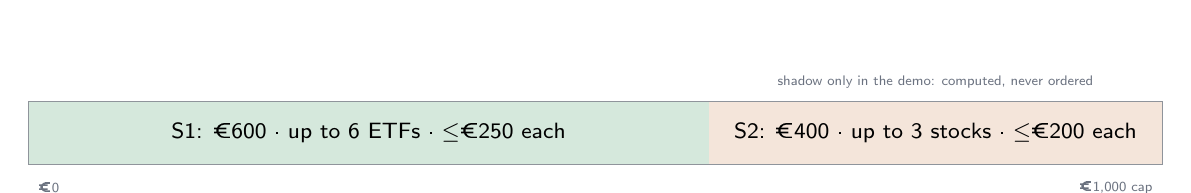
\begin{tikzpicture}
  \def\W{14.4}
  \fill[good!18] (0,0) rectangle (0.6*\W,0.8);
  \fill[warn!15] (0.6*\W,0) rectangle (\W,0.8);
  \draw[ink!50,line width=0.5pt] (0,0) rectangle (\W,0.8);
  \node[font=\sffamily\footnotesize,align=center] at (0.3*\W,0.4) {S1: \euro600 \textperiodcentered{} up to 6 ETFs \textperiodcentered{} $\le$\euro250 each};
  \node[font=\sffamily\footnotesize,align=center] at (0.8*\W,0.4) {S2: \euro400 \textperiodcentered{} up to 3 stocks \textperiodcentered{} $\le$\euro200 each};
  \node[font=\sffamily\tiny,color=muted] at (0.8*\W,1.05) {shadow only in the demo: computed, never ordered};
  \node[font=\sffamily\tiny,color=muted,anchor=west] at (0,-0.3) {\euro0};
  \node[font=\sffamily\tiny,color=muted,anchor=east] at (\W,-0.3) {\euro1,000 cap};
\end{tikzpicture}
\end{center}

% =====================================================================
\Section{Does it work? The backtest evidence}
% =====================================================================
\doc{docs/06-backtesting.md, docs/10 step 11, reports/}

\subsection{How backtests lie, and the countermeasures}
\begin{tbl}{@{}P{3.0cm}L@{}}
\TopRule
\hd{Bias} & \hd{Countermeasure} \\
\MidRule
Look-ahead & Signal on the close of day $t$, fill at the open of $t+1$; the engine only sees history up to $t$ \\
Overfitting & Few parameters; robustness grids (accept a plateau, not a spike); a holdout run once; a trial log of every run \\
Ignoring costs & A conservative cost model, and every result rerun at \textbf{2$\times$ costs} \\
Unrealistic fills & Stops fill at the stop \emph{or worse}, including gaps through the stop at the open \\
Cherry-picked regime & $\ge$ 10 years including 2008, 2020 and 2022 \\
Code drift & The same \code{Strategy}, sizing and risk code run in the backtest and live \\
LLM leakage & The LLM desk is never backtested; it is measured going forward only \\
\BotRule
\end{tbl}

\subsection{Method}
\textbf{Execution model.} Entry limit orders at the last close + 1\,\% fill at the next open only if the open is at or below the
limit. Market exits fill at the next open with slippage. Stops fill at the stop minus slippage, or at the open if it gapped
through. \textbf{Costs per side:} 0.10\,\% slippage for EU instruments; 0.05\,\% slippage plus the 0.15\,\% FX fee for US stocks.

\textbf{Data splits.} Parameters were chosen on the in-sample period, frozen, and only then was the holdout run,
\textbf{once}. The CLI enforces this: it refuses a holdout run without \code{-{}-frozen} and refuses a second one.
\begin{center}
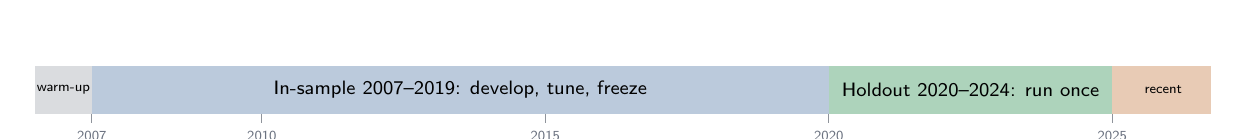
\begin{tikzpicture}[x=0.72cm]
  \fill[muted!25] (0,0) rectangle (1,0.6);
  \fill[accent!30] (1,0) rectangle (14,0.6);
  \fill[good!35] (14,0) rectangle (19,0.6);
  \fill[warn!30] (19,0) rectangle (20.75,0.6);
  \node[font=\sffamily\tiny] at (0.5,0.3) {warm-up};
  \node[font=\sffamily\scriptsize] at (7.5,0.3) {In-sample 2007--2019: develop, tune, freeze};
  \node[font=\sffamily\scriptsize] at (16.5,0.3) {Holdout 2020--2024: run once};
  \node[font=\sffamily\tiny,align=center] at (19.9,0.3) {recent};
  \foreach \y/\x in {2007/1,2010/4,2015/9,2020/14,2025/19}{
    \draw[ink!50] (\x,0) -- (\x,-0.12); \node[font=\sffamily\tiny,color=muted,below] at (\x,-0.1) {\y};}
\end{tikzpicture}
\end{center}
Every run (parameters, period, code hash, metrics) is appended to \code{data/trials.jsonl}, so the honest number of trials is
always known.

\subsection{S1 results: passes}
\begin{tbl}{@{}P{3.1cm}P{3.0cm}P{1.9cm}P{1.4cm}P{1.1cm}L@{}}
\TopRule
\hd{Period} & \hd{CAGR (1$\times$ / 2$\times$ costs)} & \hd{Sharpe} & \hd{Max DD} & \hd{Trades} & \hd{Benchmark CAGR / DD} \\
\MidRule
In-sample 2007--2019 & +3.4\,\% / +2.9\,\% & 0.45 $\pm$ 0.29 & $-$12.4\,\% & 210 & +8.6\,\% / $-$40.3\,\% \\
\textbf{Holdout 2020--2024} & \textbf{+4.5\,\% / +3.8\,\%} & \textbf{0.71} & \textbf{$-$13.4\,\%} & 89 & +10.6\,\% / $-$24.0\,\% \\
Recent 2025--Sep 2026 & +3.5\,\% / +2.7\,\% & 0.65 & $-$5.4\,\% & 27 & +16.2\,\% / $-$14.6\,\% \\
\BotRule
\end{tbl}
{\small The benchmark is the equal-weight basket of the same six ETFs, rebalanced daily, with no costs. CAGR = compound annual
growth rate; DD = drawdown from the previous peak.}

\begin{figure}[h!]
  \centering
  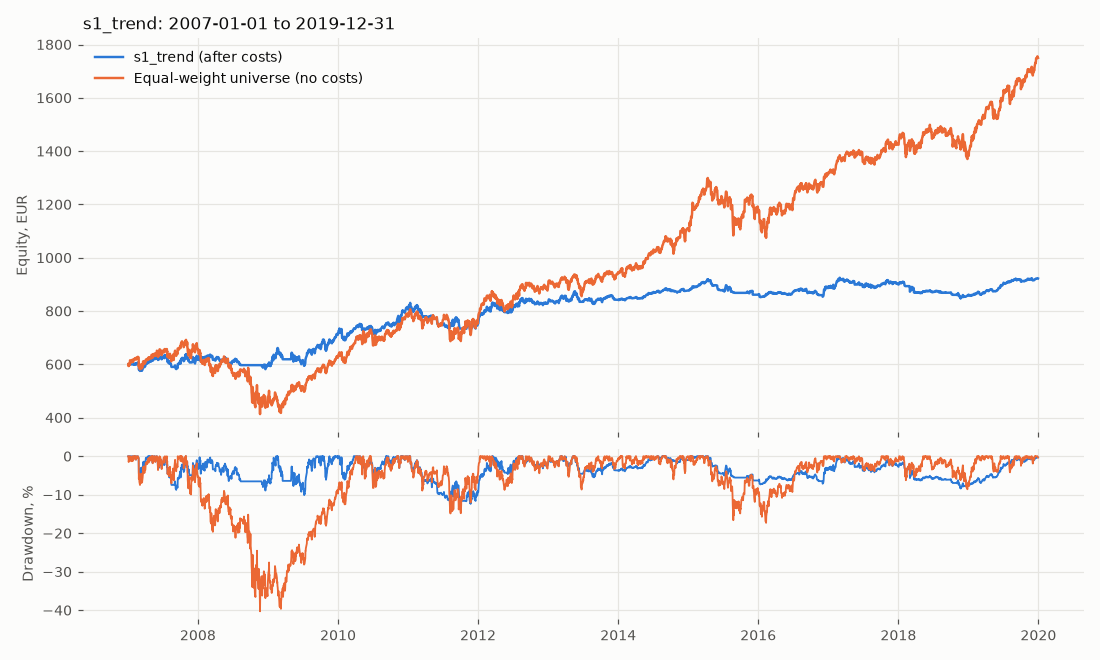
\includegraphics[width=\linewidth]{../../reports/backtest_s1_trend_insample_2026-09-25.png}
  \par\smallskip{\small\sffamily\color{muted}S1 in-sample, 2007--2019, starting from its \euro600 budget. Top: equity after
  costs (blue) versus buy-and-hold of the same six ETFs (orange). Bottom: drawdown. S1 sidesteps most of 2008 but gives up much
  of the 2012--2019 rally.}
\end{figure}

What the chart shows is S1's real character. It \textbf{cut the worst drawdown by two thirds} (in 2008: $-$2.8\,\% versus
$-$29\,\% for buy-and-hold), and in return it gave up more than half of buy-and-hold's gain in rising markets. The protective
stop makes 200 of its 210 exits; after a stop-out S1 waits for the next month-end check, so it is invested only about half the
time.

\begin{figure}[h!]
  \centering
  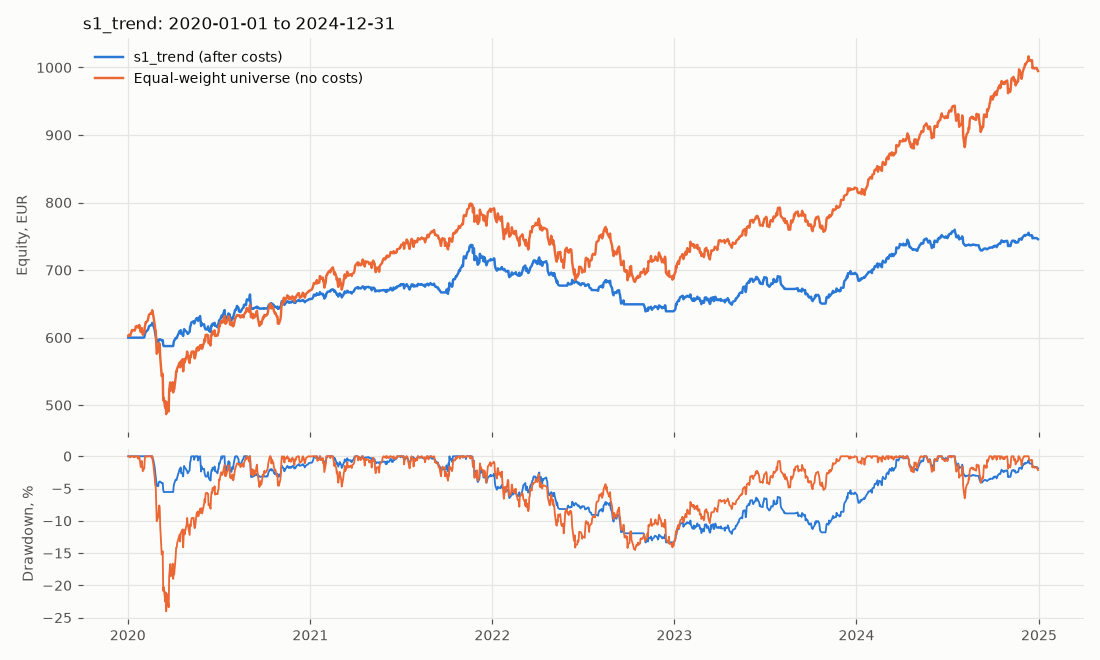
\includegraphics[width=\linewidth]{../../reports/backtest_s1_trend_holdout_2026-09-25.png}
  \par\smallskip{\small\sffamily\color{muted}S1 holdout, 2020--2024, run once after the parameters were frozen.}
\end{figure}

\textbf{Robustness.} In an 18-cell grid (SMA length, monthly versus weekly checks, stop multiple), 17 cells are profitable after
costs, and every monthly cell lands at a Sharpe of 0.42--0.61: a plateau, not a lone spike. Tighter stops scored higher
in-sample, but switching to the best cell after looking would be exactly the overfitting the method forbids, so the
pre-specified defaults were frozen.

\subsubsection{The P0 gate for S1}
\begin{tbl}{@{}LP{7.6cm}@{}}
\TopRule
\hd{Criterion} & \hd{Result} \\
\MidRule
Backtest $\ge$ 10 years where data exists & \PASS\ 13 years in-sample (with proxies) + 5 years holdout \\
Still positive at 2$\times$ costs & \PASS\ +2.9\,\% in-sample, +3.8\,\% holdout \\
Holdout Sharpe $\ge$ half the in-sample Sharpe & \PASS\ 0.71 versus 0.45 \\
Plateau in the robustness checks & \PASS\ monthly cells 0.42--0.61 \\
Max drawdown acceptable versus benchmark & \PASS\ $-$12\,\% vs $-$40\,\%; $-$13\,\% vs $-$24\,\% \\
Code unit-tested; report filed & \PASS \\
Code reviewed & \WAIT\ your review \\
\BotRule
\end{tbl}

\subsection{S2 results: fails}
\begin{tbl}{@{}P{5.2cm}P{2.6cm}P{1.3cm}P{1.5cm}L@{}}
\TopRule
\hd{Run (in-sample 2007--2019)} & \hd{CAGR (1$\times$ / 2$\times$)} & \hd{Sharpe} & \hd{Max DD} & \hd{Trades} \\
\MidRule
Default: RSI(2) $<$ 10 & $-$0.1\,\% / $-$6.0\,\% & 0.02 & $-$18.8\,\% & 935 \\
Bollinger variant (the PRD's rule) & +0.1\,\% / $-$2.2\,\% & 0.04 & $-$12.5\,\% & 395 \\
Grid, 81 cells & \multicolumn{4}{l}{35 of 81 profitable; median Sharpe $-$0.02; best 0.28} \\
\BotRule
\end{tbl}
The best grid cell is only about one standard error above zero. \textbf{Why it fails:} there is a small gross edge ($\sim$0.2\,\% per trade, 61\,\% win rate), but costs eat
\textbf{110\,\% of gross profit} at normal costs. Trades last about 3.4 days, so the spread plus the 0.3\,\% round-trip FX fee on
US names outweigh the edge. This matches the literature's warning that this edge has decayed since it was published. S2
therefore gets \textbf{no holdout run and no demo orders}; it runs in shadow, where it will be the LLM desk's test bed.

\subsection{The honest reading}\label{sec:honest}
How much can a track record tell you? The standard error of a Sharpe ratio (Lo, 2002) is roughly
\[ \mathrm{SE} \approx \sqrt{\frac{1 + \mathrm{SR}^2/2}{T}} \quad (T \text{ in years}). \]
\begin{tbl}{@{}LP{3.6cm}P{3.6cm}@{}}
\TopRule
\hd{Track record} & \hd{SE of Sharpe (at SR 0.5)} & \hd{95\,\% interval} \\
\MidRule
3 months & $\approx$ 2.1 & $-$3.7 \dots\ 4.7 \\
1 year & $\approx$ 1.06 & $-$1.6 \dots\ 2.6 \\
10 years & $\approx$ 0.34 & $-$0.2 \dots\ 1.2 \\
\BotRule
\end{tbl}
\begin{callout}{What this means for TradeBot}
\begin{itemize}
  \item S1's in-sample Sharpe of 0.45 $\pm$ 0.29 is \textbf{not statistically significant} ($t \approx 1.6$), and about 20 S1
        trials were run, which weakens it further.
  \item The robust, literature-backed property is \textbf{drawdown control}, not excess return. At \euro600, +3--4\,\% a year
        is \euro20--25 a year.
  \item Weeks or months of demo trading \textbf{cannot prove profitability}. P1 checks the \emph{implementation}: do live
        signals, fills and costs match the backtest replayed over the same days?
  \item The drawdown kill switch would have tripped twice in 18 years (2009-06-23 and 2022-05-16): roughly one pause for a
        human review every 7 years.
\end{itemize}
\end{callout}

% =====================================================================
\Section{The live engine (P1)}
% =====================================================================
\doc{docs/04-architecture.md, src/tradebot/live.py, execution.py}

\subsection{The moving parts}
\begin{center}
\begin{tikzpicture}
  \node[box=muted,minimum width=2.6cm,minimum height=2.9cm,text width=2.4cm] (ts) at (0,0) {\textbf{Windows\\Task Scheduler}\\[3pt]
     engine at boot,\\restart on failure\\[2pt] watchdog every\\minute\\[2pt] backup at 03:00};
  \node[box,minimum width=4.0cm,minimum height=2.9cm,text width=3.8cm] (en) at (6.2,0) {\textbf{Engine process}\\[3pt]
     main loop: 20 s ticks\\ sync every 2 min in session,\\ 10 min outside\\ decision cycle after the close\\
     daily report after US close\\[2pt] heartbeat thread (every 15 s)};
  \node[box=teal,minimum width=2.8cm,text width=2.6cm] (t212) at (11.4,0.8) {\textbf{Trading 212}\\practice API};
  \node[box=teal,minimum width=2.8cm,text width=2.6cm] (yh) at (11.4,-0.8) {\textbf{Yahoo}\\daily bars};
  \node[box=purple,minimum width=3.4cm,text width=3.2cm] (db) at (7.4,-2.9) {\textbf{data/demo.db} (SQLite)\\events \textperiodcentered{} orders \textperiodcentered{} lots};
  \node[box=warn,minimum width=2.8cm,text width=2.6cm] (al) at (11.4,-2.9) {\textbf{Telegram} alerts\\ \textbf{healthchecks.io} ping};
  \node[box=bad,minimum width=2.6cm,text width=2.4cm] (wd) at (0,-2.9) {\textbf{Watchdog}\\one check per run};
  \node[draw=ink!50,fill=paper,font=\sffamily\scriptsize,inner sep=3pt] (hb) at (3.0,-2.62) {\code{heartbeat.json}};
  \node[draw=bad,fill=bad!8,font=\sffamily\scriptsize,inner sep=3pt] (kill) at (3.0,-3.18) {\code{data/KILL}};
  \draw[arr] (ts) -- node[lbl,above] {starts} (en);
  \draw[arr] (ts) -- (wd);
  \draw[{Stealth[length=5pt,width=4pt]}-{Stealth[length=5pt,width=4pt]},line width=0.7pt,color=ink!80] (en.east|-t212) -- (t212);
  \draw[arr] (yh) -- (en.east|-yh);
  \draw[arr] (7.4,-1.45) -- (db.north);
  \draw[arr] (en.south east) to[out=-35,in=180] (al.west);
  \draw[arr] (4.6,-1.45) |- node[lbl,pos=0.25,left] {writes} (hb.east);
  \draw[arr] (hb.west) -- node[lbl,above] {reads} (wd.east|-hb.west);
  \draw[arr,color=bad] (wd.east|-kill) -- node[lbl,below] {trips} (kill.west);
  \draw[arr,dashed,color=bad] (kill.east) -| node[lbl,pos=0.85,right,align=left] {read before\\every order} (5.3,-1.45);
\end{tikzpicture}
\end{center}
Three scheduled tasks were installed by \code{ops/install-tasks.ps1} on 27 Sep at 23:02: the \textbf{engine} (starts at
boot, whether or not you are logged on, and restarts on failure), the \textbf{watchdog} (every minute) and the nightly
\textbf{backup}. The script also set the power plan (never sleep on AC, lid does nothing) and hourly time sync.

\subsection{A day in the life}
\begin{center}
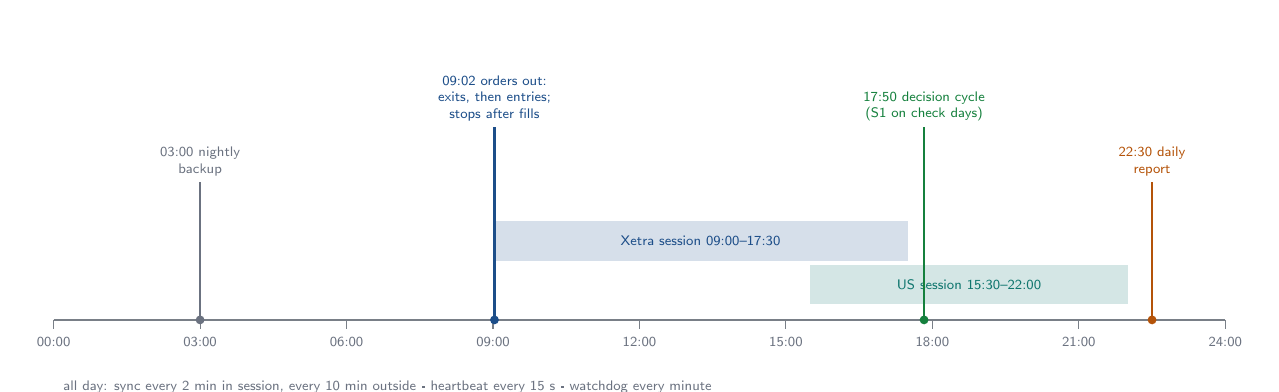
\begin{tikzpicture}[x=0.62cm]
  % sessions
  \fill[accent!18] (9,0.55) rectangle (17.5,1.05);
  \node[font=\sffamily\tiny,color=accent] at (13.25,0.8) {Xetra session 09:00--17:30};
  \fill[teal!18] (15.5,0) rectangle (22,0.5);
  \node[font=\sffamily\tiny,color=teal] at (18.75,0.25) {US session 15:30--22:00};
  % axis
  \draw[ink!60,line width=0.6pt] (0,-0.2) -- (24,-0.2);
  \foreach \h in {0,3,...,24}{\draw[ink!60] (\h,-0.2) -- (\h,-0.32); \node[font=\sffamily\tiny,color=muted,below] at (\h,-0.3) {\ifnum\h<10 0\fi\h:00};}
  % events
  \foreach \x/\y/\t/\c in {3/1.9/{03:00 nightly\\backup}/muted, 9.03/2.6/{09:02 orders out:\\exits, then entries;\\stops after fills}/accent,
                          17.83/2.6/{17:50 decision cycle\\(S1 on check days)}/good, 22.5/1.9/{22:30 daily\\report}/warn}{
    \draw[\c,line width=0.9pt] (\x,-0.2) -- (\x,\y-0.35);
    \fill[\c] (\x,-0.2) circle (1.6pt);
    \node[font=\sffamily\tiny,align=center,color=\c,anchor=south] at (\x,\y-0.4) {\t};
  }
  \node[font=\sffamily\tiny,color=muted,anchor=west] at (0,-1.05) {all day: sync every 2 min in session, every 10 min outside \textperiodcentered{} heartbeat every 15 s \textperiodcentered{} watchdog every minute};
\end{tikzpicture}
\end{center}
Times are Central European (CEST). Sessions, holidays, half days and daylight-saving changes all come from
\textbf{Trading 212's own exchange schedules}, so none of that is hard-coded. S2 is shadow-only, so P1 has no US order cycle.
\textbf{Syncs} mirror orders and fills into the ledger, reconcile against the broker, keep stops right and ping the dead-man's
switch.

\subsection{How orders are sent}
\begin{itemize}
  \item \textbf{Decisions after the close, orders at the next open + 2 minutes} (after the opening auction). Trading 212
        would queue orders placed overnight, but sending at the open means nothing except stops rests at the broker overnight,
        a crash between close and open leaves nothing half-sent, and a night-time kill has no queued entries to chase.
  \item \textbf{Entries} are DAY \textbf{limit} orders at the last close + 1\,\%: a gap up of more than 1\,\% leaves the order
        unfilled instead of paying up.
  \item \textbf{Exits} cancel the lot's stop first, then sell at market.
  \item \textbf{Protective stops} are good-till-cancelled and are placed or replaced \textbf{only while the market is open}.
        A trail decided at the close takes effect at the next open.
  \item One known difference from the backtest: an unfilled entry keeps resting for the rest of the day live, while the
        backtest counts it as unfilled at the open.
\end{itemize}
In the ledger an order moves through \code{PENDING} (planned at a close) $\to$ \code{SUBMITTING} $\to$ \code{SUBMITTED} (or
\code{UNKNOWN}) $\to$ the broker's own statuses (\code{NEW}, \code{FILLED}, \code{CANCELLED}, \code{REJECTED}, \dots). An entry fill
opens a \textbf{lot}; a stop or exit fill closes it and records the realised profit or loss.

\subsection{The submit-once protocol}\label{sec:submitonce}
Trading 212's API has no client order reference, and its docs warn that repeating a request may create a duplicate order.
So the engine \textbf{never retries an order blindly}:
\begin{center}
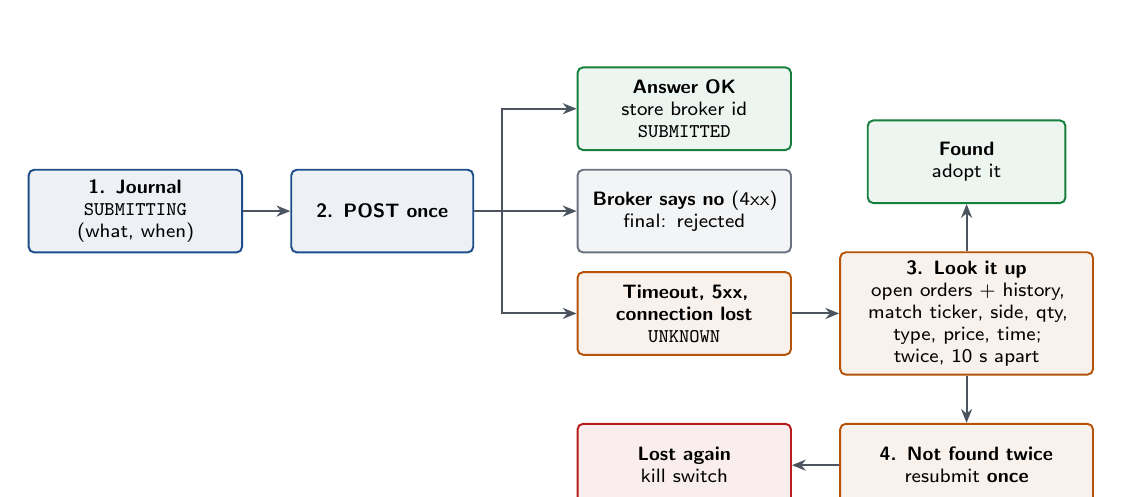
\begin{tikzpicture}[node distance=5mm and 6mm]
  \node[box,text width=2.5cm] (j) {\textbf{1. Journal}\\\code{SUBMITTING}\\(what, when)};
  \node[box,text width=2.1cm,right=of j] (p) {\textbf{2. POST once}};
  \node[box=good,text width=2.5cm,right=13mm of p,yshift=1.3cm] (ok) {\textbf{Answer OK}\\store broker id\\\code{SUBMITTED}};
  \node[box=muted,text width=2.5cm,right=13mm of p] (rej) {\textbf{Broker says no} (4xx)\\final: rejected};
  \node[box=warn,text width=2.5cm,right=13mm of p,yshift=-1.3cm] (unk) {\textbf{Timeout, 5xx,\\connection lost}\\\code{UNKNOWN}};
  \node[box=warn,text width=3.0cm,right=of unk] (look) {\textbf{3. Look it up}\\open orders + history,\\match ticker, side, qty,\\type, price, time;\\twice, 10 s apart};
  \node[box=good,text width=2.3cm,above=6mm of look] (adopt) {\textbf{Found}\\adopt it};
  \node[box=warn,text width=3.0cm,below=6mm of look] (re) {\textbf{4. Not found twice}\\resubmit \textbf{once}};
  \node[box=bad,text width=2.5cm,left=of re] (ks) {\textbf{Lost again}\\kill switch};
  \draw[arr] (j) -- (p);
  \draw[arr] (p.east) -- ++(0.35,0) |- (ok.west);
  \draw[arr] (p.east) -- (rej.west);
  \draw[arr] (p.east) -- ++(0.35,0) |- (unk.west);
  \draw[arr] (unk) -- (look);
  \draw[arr] (look) -- (adopt);
  \draw[arr] (look) -- (re);
  \draw[arr] (re) -- (ks);
\end{tikzpicture}
\end{center}
Drill 3 tested both halves live on the demo by cutting the connection at the socket. \emph{Sent, answer lost:} the lookup
found the order and adopted it, one order at the broker. \emph{Lost before sending:} two empty lookups, then exactly one
resubmit. The lookup even ignored an identical-looking order that the first case had already claimed.

\subsection{Reconciliation: the broker is the source of truth}
Every sync compares the ledger with the broker:
\begin{itemize}
  \item \textbf{Positions:} the ledger's net quantity per symbol equals the broker's.
  \item \textbf{Orders:} every open broker order is known to the ledger, and vice versa.
  \item \textbf{Stops:} every open lot has exactly one resting stop, at the right price and size. A missing stop is
        replaced automatically, with an alert; if that fails, the kill switch trips.
\end{itemize}
A mismatch must show on \textbf{two syncs in a row} before it halts trading, because Trading 212 updates order history and
positions a moment apart after a fill. An order that has left the open list but is not in history yet is ``in limbo'': its
ticker is skipped for 10 minutes, then counted as a mismatch.

\subsection{The journal}
Everything lives in \code{data/demo.db} (SQLite, WAL mode): an append-only \code{events} table (every signal, risk decision,
broker event, alert, equity mark and kill-switch change), the \code{orders} ledger and the \code{lots}. Any order can be
explained from the journal alone: data $\to$ signal $\to$ risk decision $\to$ broker events $\to$ fills. Research data stays in
\code{data/research.db}. Every run logs a \textbf{limits hash} and a \textbf{code hash}, so you can tell exactly which rules
and which code produced a decision.

\subsection{Worked example: S1's first check day}
\begin{tbl}{@{}P{3.1cm}L@{}}
\TopRule
\hd{When} & \hd{What happens} \\
\MidRule
Wed 30 Sep, $\sim$17:50 & The last Xetra session of September closes, so it is S1's monthly check day. The engine fetches fresh
  bars and requires the bar for \emph{today's} session (else it waits, then skips with an alert). For each of the six ETFs it
  computes SMA(200), ATR(20) and $\sigma_{20}$. In-trend ETFs are sized by inverse volatility within \euro600, each passes the
  risk checks, and each becomes a \code{PENDING} limit buy at close + 1\,\%. \\
Wed 30 Sep, $\sim$22:30 & The daily report lists the planned orders. \\
Thu 1 Oct, 09:02 & \code{execute\_pending} sends the orders one at a time, spaced to the rate limits, each via submit-once. \\
Thu 1 Oct, in session & Fills arrive. The sync opens a lot per fill and places a GTC stop at fill $-$ 3 $\times$ ATR, sized to
  the filled quantity. \\
Afterwards & You repeat drill 8 (delete a stop in the app; the reconciler must replace it) and the ``stops kept'' half of
  drill 1. The daily report's \textbf{forward check} replays the backtest over the live period: it must hold the same symbols as
  the engine, and any difference is flagged. \\
Fri 30 Oct & The next check day: exits for ETFs that lost the trend, stop trails, new entries. \\
\BotRule
\end{tbl}

% =====================================================================
\Section{Safety: defence in depth}
% =====================================================================
\doc{docs/05-risk-and-safety.md, src/tradebot/risk.py}

\subsection{Seven layers}
\begin{tbl}{@{}P{0.5cm}P{5.2cm}LP{2.2cm}@{}}
\TopRule
\hd{\#} & \hd{Layer} & \hd{What it stops} & \hd{Bypassable?} \\
\MidRule
1 & Strategy rules & Trades outside the rule's logic & -- \\
2 & LLM desk: reduce-only, majority of 5 (P2) & Entries into known events or bad news & can only reduce \\
3 & \textbf{Risk engine}: pre-trade checks & Any order that breaks a limit & no \\
4 & Human approval gate (P3+) & Anything you don't like & no \\
5 & Broker side: resting stops, cash account, no money-movement API & Losses while the bot is dead; money leaving & no \\
6 & Kill switch + watchdog & Trading that continues after a breach or a hang & no \\
7 & Reconciliation + daily report & Silent drift between ledger and reality & no \\
\BotRule
\end{tbl}

\subsection{The limits (\code{config/risk.toml})}\label{sec:limits}
All percentages are of \code{capital = min(broker equity, \euro1,000)}. The demo balance is far larger; the bot behaves as if it
had \euro1,000.
\begin{tbl}{@{}LP{2.2cm}P{5.4cm}@{}}
\TopRule
\hd{Limit} & \hd{Value} & \hd{On breach} \\
\MidRule
Capital cap & \euro1,000 & Reject any entry that would deploy more \\
Whitelist; long-only; no margin & 20 symbols & Reject \\
Max open positions & 9 & Reject the entry \\
Max position size & \euro250 & Reject or shrink \\
Risk per trade (entry to stop) & 0.5\,\% = \euro5 & Shrink \\
Min order & \euro20 & Reject as dust \\
Orders per day / per minute & 10 / 2 & Reject \\
Price collar (limit vs last close) & $\pm$2\,\% & Reject \\
Daily loss & 2\,\% = \euro20 & No new entries until the next session \\
Drawdown from equity peak & 10\,\% = \euro100 & \textbf{Kill switch (sticky)} \\
Consecutive broker rejects & 3 & Kill switch \\
\BotRule
\end{tbl}
Limits are read once at start, checked against bounds in code, hashed and logged. The cap's upper bound is \euro1,000
\emph{in code}, so raising it needs a code change, not a config edit. Drill 6 proved it: with \code{capital\_cap\_eur = 5000},
\code{run} refused to start. Exposure limits never block exits or stops, because those reduce risk.

\subsection{Pre-trade checks (in order; the first failure wins)}
\begin{multicols}{2}\small
\begin{enumerate}
  \item Kill switch not tripped
  \item Mode allows orders
  \item The market has a next session
  \item Symbol whitelisted and tradable
  \item No shorting: sell $\le$ held
  \item No earlier order for this intent id
  \item Rate limits (minute, day)
  \item Price fresh and sane
  \item Price collar
  \item Notional within [\euro20, \euro250]
  \item Positions, exposure, capital (entries)
  \item Daily loss state (entries)
  \item Cash available (no margin)
\end{enumerate}
\end{multicols}
Every result, pass or fail with a reason code, is journaled together with the limits hash. The unit tests give \textbf{each}
rejection reason its own failing case.

\subsection{The kill switch}
\textbf{Triggers.} Automatic: the drawdown limit; 3 broker rejects in a row; a reconciliation mismatch; an order lost twice;
bad data on a held symbol; any exception inside the risk engine. Manual: \code{kill}. Watchdog: a stale heartbeat.

\textbf{What HALT does, in this order:}
\begin{enumerate}
  \item Writes \code{data/KILL} (reason, time, who) and a journal event \textbf{before anything else}.
  \item Cancels all open \textbf{entry} orders.
  \item \textbf{Keeps the protective stops.}
  \item Blocks all new entries, and alerts you.
\end{enumerate}
\textbf{FLATTEN} (\code{kill -{}-flatten}) additionally plans a market exit for every lot at the next open. The switch is
\textbf{sticky}: it survives restarts, and it never resets itself. \code{reset-kill} shows why it tripped, requires you to type
\code{RESET}, logs who reset it and why, and the engine reconciles again before it trades.
\begin{callout}[bad]{Why the kill switch keeps the stops}
The reference PRD's kill switch ``cancels all pending orders''. That would remove the protective stops and leave every
position unprotected at exactly the moment something is broken. Here, the switch stops \emph{new risk} and leaves the
existing safety net in place.
\end{callout}

\subsection{Watchdog and dead-man's switch}
A thread in the engine rewrites \code{data/heartbeat.json} every 15 seconds, \emph{but only while the main loop has made
progress in the last 10 minutes}. The watchdog, a separate process run every minute, trips the kill switch through its own
broker session if the heartbeat is older than 60 seconds. Drill 2 killed the engine at 16:19:08 UTC; the watchdog tripped at
16:20:10, 62 seconds later. A clean \code{stop} marks the heartbeat ``stopped'' so the watchdog leaves it alone.

An on-host watchdog can't report that the whole laptop is dead. So every sync also pings \textbf{healthchecks.io} (period
10 min, grace 10 min); a missed ping alerts you by Telegram or e-mail even if the house has lost power. Telegram carries all
other alerts (each distinct text at most once an hour).

\subsection{Secrets and live arming}
\begin{itemize}
  \item Demo keys live in the git-ignored \code{.env}. \textbf{Live keys never go in \code{.env}} and never on the laptop:
        they are created only at P3, only on the VPS, and IP-restricted to its address.
  \item The Trading 212 API has no deposit or withdrawal endpoints at all.
  \item The adapter refuses any base URL but the demo. Live trading will need \textbf{three independent keys}:
        \code{mode = "live"}, the environment variable \code{TRADEBOT\_LIVE=I\_ACCEPT\_REAL\_MONEY\_RISK}, and a live key in
        the VPS's secret store.
\end{itemize}

\subsection{The drills}
\begin{tbl}{@{}P{0.8cm}P{4.4cm}LP{2.7cm}@{}}
\TopRule
\hd{\#} & \hd{Drill} & \hd{Result on the demo (27 Sep)} & \hd{Status} \\
\MidRule
1 & Manual kill with orders open & Entry cancelled at the broker, stayed halted after restart; found a bug (below) & \PASS\ (stops: after first fill) \\
2 & Kill the engine process & Watchdog tripped after 62 s & \PASS \\
3 & Network cut during a submit & No duplicate orders in either case & \PASS \\
4 & Stale data & Unit test only so far & \WAIT \\
5 & Manual order in the account & Mismatch seen once, HALT on the next sync, stray order cancelled & \PASS \\
6 & Out-of-bounds limit & \code{run} refused to start & \PASS \\
7 & LLM invalid output, timeout, injection & Needs the desk & \LATER\ P2 \\
8 & Delete a protective stop & Needs a position & \WAIT\ after 1 Oct \\
9--10 & LLM keys revoked; LLM budget exhausted & Need the desk & \LATER\ P2 \\
\BotRule
\end{tbl}

\subsection{What the tests and drills have caught so far}
\begin{tbl}{@{}P{6.6cm}L@{}}
\TopRule
\hd{Problem} & \hd{Fix} \\
\MidRule
Entries sized on the close could fill 1\,\% higher and exceed a cap (\euro202 vs \euro200) & Size and check at the limit price \\
A filled order vanishes from the active list; it would have been mistaken for a failure, leaving a position open & Read the final status from order history \\
Yahoo's Friday bar had no close on Saturday; decisions would silently use Thursday & Require the bar of the last completed session \\
Drill 1: the \code{kill} process hit HTTP 429 twice and crashed before cancelling the entry (the switch was already written, so trading was halted anyway) & Up to 3 retries on 429 with a margin; regression test \\
Git rewrote \code{risk.toml} with CRLF line endings, changing the limits hash with identical limits & Hashes ignore line endings; test added \\
\BotRule
\end{tbl}

% =====================================================================
\Section{The multi-model LLM desk (P2, not built yet)}\label{sec:desk}
% =====================================================================
\doc{docs/08-multi-agent-llm.md}

\begin{plainbox}[warn]
\small\textsf{\bfseries\color{warn}Status.} Designed, not built. It arrives in P2, in \textbf{shadow} only
(\code{affects\_orders = false}): it reviews S2's shadow entries and its value is measured before it may touch an order.
LLM spend so far: \euro0.
\end{plainbox}

\subsection{The roster}
One model per lab, so errors are as independent as possible and one provider's outage can't stop the desk.
\begin{tbl}{@{}P{2.6cm}P{4.4cm}L@{}}
\TopRule
\hd{Seat} & \hd{Default model} & \hd{Why} \\
\MidRule
Juror 1 & Claude Opus 5 (Opus 5.5 is a one-line swap) & Top lab, reliable structured output \\
Juror 2 & GPT-6 Sol & Second lab; a fifth of Astra's price \\
Juror 3 & Gemini 3.8 Flash & Third lab; fast and cheap \\
Juror 4 & GLM-5.3 (open-weight) & Top open-weight model \\
Juror 5 & Kimi K3 (open-weight) & Top open-weight model, different lab \\
News analyst & DeepSeek V4.1 Flash & Cheapest capable model; the only seat that reads raw news \\
Reporter & Gemini 3.8 Flash & Writes explanations; decides nothing \\
\BotRule
\end{tbl}
Paid labs are called through their native SDKs; open-weight models through OpenRouter with zero data retention.
\textbf{No LiteLLM}: its package was compromised in a supply-chain attack in March 2026.

\subsection{The pipeline for one entry}
\begin{center}
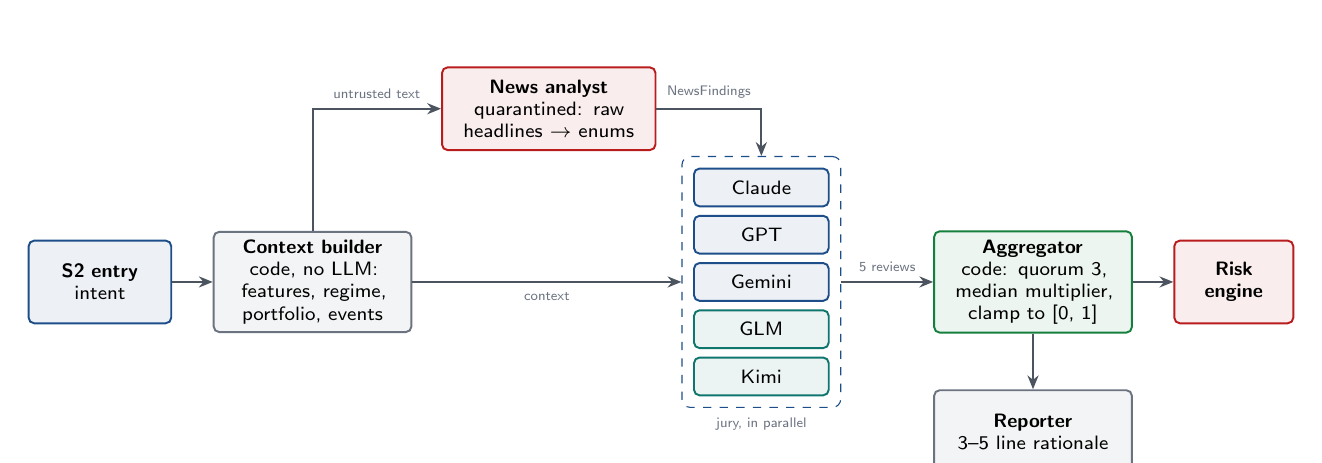
\begin{tikzpicture}
  \node[box,text width=1.6cm] (in) at (0.9,0) {\textbf{S2 entry}\\intent};
  \node[box=muted,text width=2.3cm] (cb) at (3.6,0) {\textbf{Context builder}\\code, no LLM:\\features, regime,\\portfolio, events};
  \node[box=bad,text width=2.5cm] (na) at (6.6,2.2) {\textbf{News analyst}\\quarantined: raw\\headlines $\to$ enums};
  \foreach \n/\y/\c in {Claude/1.2/accent,GPT/0.6/accent,Gemini/0/accent,GLM/-0.6/teal,Kimi/-1.2/teal}
    \node[box=\c,minimum height=0.48cm,text width=1.5cm] (\n) at (9.3,\y) {\n};
  \node[draw=accent,dashed,rounded corners=3pt,inner sep=4pt,fit=(Claude)(Kimi),label={[lbl]below:{jury, in parallel}}] (jury) {};
  \node[box=good,text width=2.3cm] (ag) at (12.75,0) {\textbf{Aggregator}\\code: quorum 3,\\median multiplier,\\clamp to [0, 1]};
  \node[box=bad,text width=1.3cm] (re) at (15.3,0) {\textbf{Risk}\\\textbf{engine}};
  \node[box=muted,text width=2.3cm] (rp) at (12.75,-1.9) {\textbf{Reporter}\\3--5 line rationale};
  \draw[arr] (in) -- (cb);
  \draw[arr] (cb.north) |- node[lbl,pos=0.75,above] {untrusted text} (na.west);
  \draw[arr] (na.east) -| node[lbl,pos=0.25,above] {NewsFindings} (jury.north);
  \draw[arr] (cb.east) -- node[lbl,below] {context} (jury.west|-cb.east);
  \draw[arr] (jury.east|-ag.west) -- node[lbl,above] {5 reviews} (ag.west);
  \draw[arr] (ag) -- (re);
  \draw[arr] (ag) -- (rp);
\end{tikzpicture}
\end{center}
\begin{enumerate}
  \item \textbf{Context builder (code).} Whatever code can compute, code computes: price features, a deterministic market
        regime, portfolio weights, the next earnings date, and headlines from allow-listed sources only.
  \item \textbf{News analyst (quarantine).} The only agent that sees raw internet text. It returns \code{NewsFindings}, mostly
        enums with $\le$200-character summaries, so instructions hidden in a headline have nowhere to travel.
  \item \textbf{Jury.} Five models, called independently with the same versioned prompt, each returning a validated
        \code{Review}: approve, reduce or veto, a size multiplier in [0, 1], a confidence, risk flags and a short rationale.
        The prompt tells jurors to approve unless the context gives a \emph{concrete} reason, so they don't veto everything
        out of caution.
  \item \textbf{Aggregator (code, not an LLM ``chair'').} Deterministic, auditable, robust to one bad model.
  \item \textbf{Reporter.} Writes the explanation for reports and approval prompts from the structured outputs only.
\end{enumerate}

\subsection{How the vote works}
A veto counts as a multiplier of 0. The final multiplier is the \textbf{median} of the valid reviews, so a veto needs a majority
and no single model can decide.
\begin{tbl}{@{}P{5.8cm}P{3.4cm}L@{}}
\TopRule
\hd{Five reviews (multipliers)} & \hd{Median} & \hd{Outcome} \\
\MidRule
1.0, 1.0, 0.5, 1.0, \textbf{0 (veto)} & 1.0 & Full size: one veto can't block \\
1.0, 0.6, 0.5, 0, 0 & 0.5 & Half size \\
0, 0, 0, 1.0, 1.0 & 0 & Vetoed by a majority \\
Only 2 valid reviews (3 timed out) & -- & Quorum failed: entry vetoed (\code{desk\_unavailable}) in live-affecting mode; unchanged in shadow \\
Two or more jurors flag \code{data\_suspect} & -- & Entry skipped, you are alerted \\
\BotRule
\end{tbl}

\subsection{Measuring whether it helps}
The desk can't be backtested, so it is measured forward, in shadow, with \textbf{counterfactual books} that cost nothing extra
once the signals exist: \textbf{A} = strategies only; \textbf{B} = strategies + desk; \textbf{J1--J5} = strategies + one juror
alone. Per juror: veto and reduce rates, \emph{veto precision} (vetoed entries that would have lost, versus the base loss rate),
agreement with the majority, calibration, failure rate, latency and cost. The desk may affect orders only with $\ge$ 50 reviewed
entries, veto precision above the base loss rate, a book-B drawdown no worse than A's, and a cost that pays for itself.
``The LLMs don't help'' is an acceptable research result.

\subsection{Cost}
About \textbf{\$0.18 per review} for all six seats (Claude $\approx$\$0.075, Kimi $\approx$\$0.045, GPT $\approx$\$0.03, GLM
$\approx$\$0.016, Gemini $\approx$\$0.011, DeepSeek $\approx$\$0.004). Budgets are hard caps enforced in three places (engine,
prepaid credits, provider alerts): \euro10/month for runtime, \euro15/month for offline evaluation. When the runtime budget runs
out, the desk switches off and the strategies run alone. Against a \euro1,000 cap even \euro3 a month is $\sim$4\,\% a year, more
than a realistic edge, so desk spend is reported as a research cost.

\subsection{Interim: Claude seats on your Claude subscription}
Until API keys exist, the Claude juror (and reporter) can run through Claude Code in headless mode (\code{claude -p}), locked
down: empty working directory, no user settings, no MCP servers or connectors, no tools, one turn, the juror prompt as system
prompt and the \code{Review} schema as output. The adapter reads the session's init report and \textbf{discards the result unless
the tool, MCP-server and plugin lists are all empty}. One juror alone can't reach the quorum, so this only serves shadow mode.

% =====================================================================
\Section{Hosting}
% =====================================================================
\doc{docs/09-hosting.md}

\textbf{Now (P0--P2): this laptop, 24/7.} An Intel i5-7200U (2 cores), 7.9\,GB RAM, no usable GPU. Plenty for the engine (plain
REST calls and a small SQLite file), useless for local LLMs, which is why open-weight models run on hosted inference. Electricity
is about \euro35--50 a year.
\begin{tbl}{@{}P{5.4cm}L@{}}
\TopRule
\hd{Risk on a home laptop} & \hd{Mitigation} \\
\MidRule
Windows Update reboots & Active hours around the cycles (\WAIT\ you); engine restarts at boot; startup reconciliation resumes cleanly \\
Sleep, hibernate, lid closed & Power plan set by the install script \\
Power or internet outage & Stops rest at the broker; healthchecks.io alerts you \\
Shared personal machine & Acceptable for \textbf{demo keys only} \\
\BotRule
\end{tbl}
\textbf{Before real money (P3): a small EU VPS} (1--2 vCPU, 2--4\,GB RAM, $\approx$\euro5--10/month). Always on, datacentre
power, snapshots, a single-purpose machine for the live keys with an IP-restricted key, systemd services with
\code{Restart=always}, and drill 2 repeated there.

% =====================================================================
\clearpage
\Section{The code}
% =====================================================================
\doc{docs/04 §10--11}

\subsection{Modules}
\begin{tbl}{@{}P{2.6cm}P{1.0cm}LP{1.2cm}@{}}
\TopRule
\hd{File} & \hd{Lines} & \hd{Role} & \hd{Phase} \\
\MidRule
\code{models.py} & 78 & Data contracts: \code{Signal}, \code{OrderIntent}, \code{RiskDecision}, \code{Trade}, \code{Position}; deterministic intent ids & P0 \\
\code{config.py} & 69 & Loads the TOML files, checks bounds, hashes them & P0 \\
\code{data.py} & 247 & Yahoo, Alpaca and FX downloads; cache; validation; proxy stitching; EUR panels & P0 \\
\code{indicators.py} & 45 & SMA, ATR, RSI, Bollinger, volatility (Wilder smoothing where standard) & P0 \\
\code{strategies.py} & 127 & S1 and S2: \code{features()} and a pure \code{decide()} & P0 \\
\code{sizing.py} & 33 & Budgets, inverse volatility, risk-based sizing, caps, order intents & P0 \\
\code{sim.py} & 38 & Simulated fills and the cost model & P0 \\
\code{risk.py} & 111 & The 13 pre-trade checks and the kill switch & P0 \\
\code{backtest.py} & 203 & Daily event loop and metrics & P0 \\
\code{report.py} & 157 & Markdown reports, charts, Monte Carlo, trial log & P0 \\
\code{trading212.py} & 184 & REST adapter (demo only), rate limits, calendar from exchange schedules & P1 \\
\code{execution.py} & 329 & Order manager: submit-once, sync, fills $\to$ lots, stops, reconciler, HALT & P1 \\
\code{live.py} & 394 & Engine loop, decision cycle, heartbeat, watchdog check, equity marks, daily report & P1 \\
\code{store.py} & 62 & SQLite journal and ledger & P1 \\
\code{notify.py} & 38 & Console, Telegram, healthchecks.io & P1 \\
\code{cli.py} & 305 & The command line (Section~\ref{sec:ops}) & P0--P1 \\
\BotRule
\end{tbl}
Planned for P2: \code{llm\_providers.py} (about 30 lines per provider) and \code{desk.py} (context builder, news analyst, jury,
aggregator, reporter).

\subsection{Tests}
82 tests, all passing: risk 17, execution 14, config 9, live 7, strategies 7, indicators 6, Trading 212 adapter 6, sizing 5,
backtest 4, simulator 4, data 3. The execution and live tests run against a \textbf{stateful fake Trading 212}, including a
full loop: month-end close $\to$ planned entry $\to$ sent at the open $\to$ fill $\to$ stop at fill $-$ 3 ATR $\to$ stop-out
closes the lot $\to$ reconciliation OK. A test fixture keeps every test away from the real \code{data/KILL}.

\subsection{Configuration and data files}
\begin{tbl}{@{}P{4.4cm}L@{}}
\TopRule
\hd{File} & \hd{Content} \\
\MidRule
\code{config/settings.toml} & Mode (\code{demo}), live start date, which strategies trade or shadow, budgets, cost model, test periods \\
\code{config/risk.toml} & The limits (Section~\ref{sec:limits}), reviewed separately \\
\code{config/instruments.toml} & The 20 instruments: ISIN, market, currency, data symbols, proxy, \code{native\_from} \\
\code{config/t212\_tickers.toml} & Symbol $\to$ Trading 212 ticker, generated from ISINs \\
\code{data/} (git-ignored) & \code{demo.db}, \code{research.db}, \code{trials.jsonl}, \code{heartbeat.json}, \code{KILL}, \code{kill\_log.jsonl}, \code{engine.log} \\
\code{reports/} & Backtest reports and charts, grids, the data check, \code{daily/} reports \\
\BotRule
\end{tbl}

\subsection{Technology choices}
Python 3.13, managed by \code{uv} with a lockfile that pins every package by hash (supply-chain hygiene). Runtime dependencies
are only \code{pandas}, \code{numpy} and \code{matplotlib}; everything else is standard library: \code{urllib} for Trading 212,
Yahoo, Alpaca, Telegram and healthchecks; \code{sqlite3}; \code{tomllib}; \code{argparse}. No TA library (each indicator is a
few lines), no scheduler framework (a simple loop plus Task Scheduler), no dashboard (the daily report and \code{status} are
enough).

% =====================================================================
\Section{Operating it}\label{sec:ops}
% =====================================================================
\doc{docs/04 §9 and §12}

Run from \code{D:\textbackslash TradeBot} as \code{uv run python -m tradebot <command>}.
\begin{tbl}{@{}P{5.2cm}L@{}}
\TopRule
\hd{Command} & \hd{What it does} \\
\MidRule
\code{status} & Mode, kill switch, heartbeat, last reconciliation, equity, open lots and orders, recent alerts \\
\code{stop} & Asks the running engine to exit cleanly within 20 s (any other way looks like a crash and trips the switch) \\
\code{kill -{}-reason "..."} & HALT: cancel entries, keep stops, block new entries \\
\code{kill -{}-flatten -{}-reason "..."} & Also plan a market exit for every lot at the next open \\
\code{reset-kill -{}-who .. -{}-reason ..} & Shows why it tripped; you type \code{RESET}; logged \\
\code{reconcile} & Reconcile on demand (engine stopped) \\
\code{report} & Write the daily report now \\
\code{run} / \code{watchdog} & Start the engine / one watchdog check (normally Task Scheduler does both) \\
\code{data} / \code{backtest} / \code{grid} & Refresh research data; run a backtest (\code{-{}-strategy s1 -{}-period insample}); run a robustness grid \\
\BotRule
\end{tbl}

\subsection{Short runbook}
\begin{tbl}{@{}P{4.2cm}L@{}}
\TopRule
\hd{Situation} & \hd{Action} \\
\MidRule
Start of day & \code{status}: kill switch off, heartbeat fresh, reconciliation OK \\
Kill switch tripped & Read the reason (\code{status} or journal) $\to$ fix the cause $\to$ \code{reconcile} $\to$ \code{reset-kill} \\
Engine crashed mid-cycle & Let Task Scheduler restart it. Startup reconciliation resolves \code{SUBMITTING}/\code{UNKNOWN} orders. Never resubmit by hand without checking the broker's open orders. \\
Broker API down & The engine backs off and halts entries; the stops at the broker still protect positions \\
Unexpected position at the broker & The kill switch trips automatically. Was it a manual trade in the bot's account? That is not allowed. \\
\BotRule
\end{tbl}
\begin{callout}[warn]{One rule for you}
Don't trade by hand in the bot's Trading 212 practice account. The engine treats any position or order it didn't create as a
mismatch and halts, which is exactly what drill 5 demonstrated. Keep manual investing at another broker.
\end{callout}
Where to look: Telegram for alerts; \code{reports/daily/<date>.md} after each US close; \code{status} any time;
\code{data/engine.log} for detail.

% =====================================================================
\Section{Roadmap and what happens next}\label{sec:roadmap}
% =====================================================================
\doc{docs/07-roadmap.md, docs/10-build-log.md}

\begin{center}
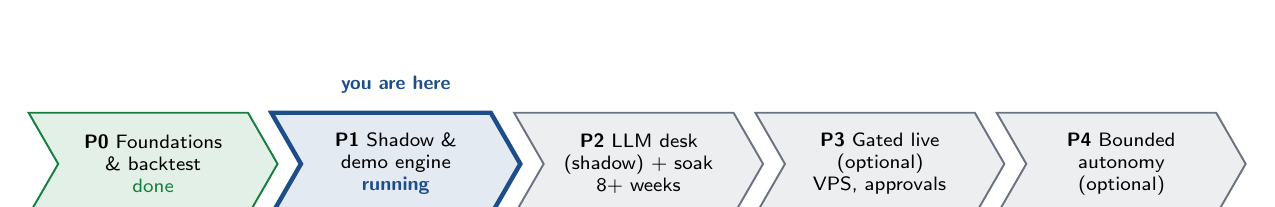
\begin{tikzpicture}[
  ph/.style={draw=#1,fill=#1!12,line width=0.7pt,shape=signal,signal to=east,signal from=west,signal pointer angle=120,
             minimum height=1.3cm,text width=2.2cm,align=center,font=\sffamily\scriptsize,inner sep=3pt},
  node distance=2.5mm]
  \node[ph=good] (p0) {\textbf{P0} Foundations\\ \& backtest\\\textcolor{good}{done}};
  \node[ph=accent,right=of p0,line width=1.6pt] (p1) {\textbf{P1} Shadow \&\\demo engine\\\textcolor{accent}{\textbf{running}}};
  \node[ph=muted,right=of p1] (p2) {\textbf{P2} LLM desk\\(shadow) + soak\\8+ weeks};
  \node[ph=muted,right=of p2] (p3) {\textbf{P3} Gated live\\(optional)\\VPS, approvals};
  \node[ph=muted,right=of p3] (p4) {\textbf{P4} Bounded\\autonomy\\(optional)};
  \node[font=\sffamily\scriptsize\bfseries,color=accent,above=1mm of p1] {you are here};
\end{tikzpicture}
\end{center}

\begin{tbl}{@{}P{1.0cm}LP{5.8cm}@{}}
\TopRule
\hd{Phase} & \hd{Deliverables} & \hd{Exit gate} \\
\MidRule
P0 & Data, indicators, S1/S2, sizing, simulator, backtester, risk engine, trial log & \PASS\ ``Idea $\to$ Demo'' for at least one strategy (S1) \\
P1 & Trading 212 adapter, order manager, stops, reconciler, kill switch, watchdog, alerts, daily report & 2 weeks of clean unattended runs; drills 1--8 \\
P2 & Provider adapters, news sources, desk, eval set, injection tests, books A/B/J; $\ge$ 8 weeks of demo & 100\,\% signal match with the backtest replay; slippage within the model; zero unexplained orders; all drills; VPS; \textbf{your decision} to use real money \\
P3 & VPS, live keys, Telegram approvals, live arming & $\ge$ 4 weeks live with every order approved, zero breaches; your decision \\
P4 & Approval only above thresholds & Ongoing; stop on the drawdown kill switch or 3 months worse than the backtest \\
\BotRule
\end{tbl}
The project is complete and useful as a research system at the end of P2. P3 and P4 are optional.

\subsection{Coming up}
\begin{tbl}{@{}P{3.3cm}L@{}}
\TopRule
\hd{When} & \hd{What} \\
\MidRule
Mon 28 Sep & The demo run officially starts. The engine syncs, pings and reports daily. \\
Wed 30 Sep, $\sim$17:50 & S1's first check day: signals, sizing, risk checks, entries planned \\
Thu 1 Oct, $\sim$09:02 & First orders go out; fills; stops follow. Then drill 8 and the ``stops kept'' half of drill 1. \\
$\sim$mid-October & P1 gate review. ``Clean'' means no kill-switch trip or mismatch caused by an engine fault, a daily report for
                    every US session, and a matching forward check. \\
Fri 30 Oct & Next S1 check day: exits, stop trails, new entries \\
\BotRule
\end{tbl}

\subsection{What needs you}
\begin{enumerate}
  \item \textbf{Set Windows Update active hours} to 06:00--00:00, so an update never reboots the laptop mid-cycle.
  \item \textbf{Review the three P1 defaults} (Section~\ref{sec:defaults}): S2 shadow-only, its \euro400 unused, Yahoo for EU data.
  \item \textbf{Review the code} (the last open item of the P0 gate).
  \item At the start of P2: create the LLM provider accounts and keys (Anthropic, OpenAI, Google, OpenRouter), each with a hard
        spend cap in its console.
\end{enumerate}

\subsection{What could change the plan}
\begin{tbl}{@{}P{5.5cm}L@{}}
\TopRule
\hd{Risk} & \hd{Answer} \\
\MidRule
A strategy fails its gate & A valid research result: keep the pipeline, try the next family \\
The demo phase is slow (S1 trades a few times a quarter) & S2's shadow decisions keep the desk's evaluation going \\
Trading 212's beta API changes or falls short & The adapter is isolated; IBKR is the documented fallback \\
The free EU data source breaks & Cross-checks and freshness checks catch it; EODHD is the paid upgrade \\
LLM model churn & The roster lives in config; the eval set runs before any swap \\
Scope creep & Nothing extra before the P2 gate \\
\BotRule
\end{tbl}

% =====================================================================
\Section{Glossary}
% =====================================================================
\begin{description}[style=nextline,leftmargin=1.4em,font=\sffamily\bfseries\color{accent},itemsep=3pt]
\small
  \item[Adjusted price] A price history corrected for splits and dividends; signals use it, order sizes use raw prices.
  \item[ATR] Average true range: the typical daily price range. Stops are set a multiple of it away.
  \item[Backtest] Running a strategy over historical data with a realistic fill and cost model.
  \item[Book (counterfactual)] A simulated portfolio showing what \emph{would} have happened under a given rule set (A, B, J1--J5).
  \item[Check day] The last trading day of the month, when S1 looks at its signals.
  \item[Dead-man's switch] An external service that alerts when the engine's regular ping stops arriving (healthchecks.io).
  \item[Drawdown] The fall from the highest equity so far. The 10\,\% limit trips the kill switch.
  \item[Drill] A deliberate failure (killing the engine, cutting the network, a stray order) to prove a safety mechanism works.
  \item[GTC / DAY] Order validity: good-till-cancelled (stops) or for the current session only (entries).
  \item[HALT / FLATTEN] The kill switch's two modes: stop new risk and keep stops / additionally close every position.
  \item[Holdout] Data kept unseen during development and tested once, after parameters are frozen.
  \item[Intent] A sized, not-yet-sent order derived from a signal, with a deterministic id so it can never be sent twice.
  \item[Journal] The append-only event log in SQLite that explains every decision and order.
  \item[Kill switch] A sticky halt flag in \code{data/KILL}, read before every order, reset only by a human.
  \item[Lot] One strategy's position from one entry fill, with its own stop and realised P\&L.
  \item[Proxy] A long-history stand-in (the US twin in EUR) for a UCITS ETF before it existed or before its data is trusted.
  \item[Quorum / median] The desk needs 3 valid reviews; the final size multiplier is their median.
  \item[Reconciliation] Comparing the ledger with the broker's positions, orders and stops; a persistent mismatch halts trading.
  \item[Reduce-only] The LLM desk may shrink or veto an entry, never enlarge it or touch an exit.
  \item[RSI] Relative strength index; RSI(2) below 10 marks a sharp two-day drop.
  \item[Shadow mode] Decisions are computed and journaled but no order is sent (S2 in P1; the desk in P2).
  \item[Sharpe ratio] Annual return divided by annual volatility; noisy over short periods (Section~\ref{sec:honest}).
  \item[SMA] Simple moving average; SMA(200) is the long-term trend line.
  \item[Submit-once] The rule that an order request is never retried blindly, because Trading 212 has no duplicate protection.
  \item[UCITS ETF] An EU-regulated fund; the only kind of ETF EU retail investors can buy.
  \item[Watchdog] A separate process that trips the kill switch when the engine's heartbeat goes stale.
  \item[ZDR] Zero data retention: providers that keep nothing from requests (OpenRouter setting).
\end{description}

% =====================================================================
\appendix
\Section{Tax and legal notes (not advice)}\label{app:tax}
% =====================================================================
\doc{docs/05 §12}
\begin{itemize}
  \item \textbf{Tax.} Capital gains, dividends and interest are taxed at the flat 25\,\% Abgeltungsteuer plus the 5.5\,\%
        solidarity surcharge on it ($\approx$26.4\,\%, plus church tax if applicable); the Sparer-Pauschbetrag exempts \euro1,000
        a year. \textbf{Trading 212 has withheld this automatically since 5 January 2026} (its German accounts run through a
        partnership with FXFlat). Losses on shares only offset gains on shares; equity ETFs get a 30\,\% partial exemption; US
        dividends carry 15\,\% US withholding with a W-8BEN on file, creditable against German tax. Confirm specifics with a
        Steuerberater.
  \item \textbf{Broker terms.} Only official APIs, as documented; the main reason Trade Republic is excluded from automation.
  \item \textbf{MiFID II} algorithmic-trading obligations fall on investment firms, not on a private individual trading their
        own account. Re-assess if the system ever trades for others.
  \item \textbf{EU AI Act} Article 2(10) excludes natural persons using AI in a purely personal, non-professional activity.
  \item \textbf{The US pattern-day-trader rule} does not apply: it targets US margin accounts.
\end{itemize}

\Section{Where to read more}
\begin{tbl}{@{}P{4.8cm}L@{}}
\TopRule
\hd{Repository document} & \hd{Covers} \\
\MidRule
\code{README.md} & Summary, key decisions D1--D10, PRD differences, resolved items \\
\code{docs/01-platforms.md} & Brokers, data sources, the Germany specifics, Trading 212 API facts \\
\code{docs/02-approaches.md} & Rules vs ML vs RL vs LLM trader vs hybrid; the LLM's allowed role \\
\code{docs/03-strategies.md} & Strategy families surveyed; S1 and S2 full specs; costs \\
\code{docs/04-architecture.md} & Components, runtime cycle, data contracts, order lifecycle, config, CLI, stack \\
\code{docs/05-risk-and-safety.md} & Limits, checks, kill switch, watchdog, reconciliation, failure modes, drills, tax \\
\code{docs/06-backtesting.md} & Biases, method, metrics, statistics, desk evaluation, promotion gates \\
\code{docs/07-roadmap.md} & Phases, P0 backlog, Trading 212 API questions and answers \\
\code{docs/08-multi-agent-llm.md} & Model landscape, roster, pipeline, providers, cost, evaluation \\
\code{docs/09-hosting.md} & Laptop vs VPS, checklists \\
\code{docs/10-build-log.md} & What was built, step by step: decisions, findings, bugs, results \\
\code{reports/} & Backtest reports and charts, robustness grids, data check, daily reports \\
\BotRule
\end{tbl}

\end{document}
